\documentclass[tikz]{standalone}
\usepackage{pgfplots}
\pgfplotsset{compat=1.15}
\usepackage{mathrsfs}
\usetikzlibrary{arrows,calc}
\usepackage{tkz-euclide}

\pagestyle{empty}

\definecolor{AngleClr}{rgb}{0,0.39215686274509803,0}
\definecolor{ShapeClr}{rgb}{0.6,0.2,0}
\definecolor{SecondAngleClr}{RGB}{14, 70, 161}

\begin{document}

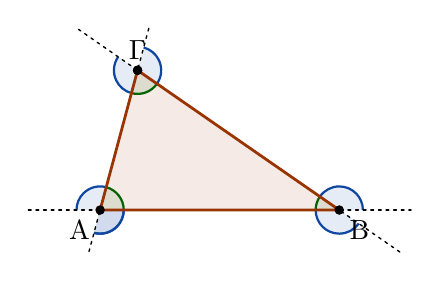
\begin{tikzpicture}[scale=.75]
\tkzSetUpLine[line width=1pt,color=black]
\tkzSetUpPoint[fill=black]

\tkzDefPoints{0/0/B,4.05/0/C}

\tkzDefPoint(75:2.45){A}
\tkzDefPoint(75:2.45){D}

\tkzDefPointOnLine[pos=1.2](A,B)\tkzGetPoint{A1}
\tkzDefPointOnLine[pos=-0.2](A,B)\tkzGetPoint{A2}
\tkzDefPointOnLine[pos=1.2](B,C)\tkzGetPoint{B1}
\tkzDefPointOnLine[pos=-0.2](B,C)\tkzGetPoint{B2}
\tkzDefPointOnLine[pos=1.2](C,A)\tkzGetPoint{C1}
\tkzDefPointOnLine[pos=-0.2](C,A)\tkzGetPoint{C2}

\tkzFillPolygon[fill=ShapeClr,fill opacity=0.1](A,B,C,D)

% Internal angles.
\tkzFillAngles[fill=AngleClr,size=.4,fill opacity=0.1](C,B,A A,C,B B,A,C)
\tkzMarkAngles[line width=0.8pt,size=.4,color=AngleClr](C,B,A A,C,B B,A,C)

% External angles.
\tkzFillAngles[fill=SecondAngleClr,size=.4,fill opacity=0.1](A,B,B2 A1,B,C A1,B,C B,C,C2 C,A,A2 C1,A,B B1,C,A)
\tkzMarkAngles[line width=0.8pt,size=.4,color=SecondAngleClr](A,B,B2 A1,B,C A1,B,C B,C,C2 C,A,A2 C1,A,B B1,C,A)

\tkzDrawSegments[line width=0.5pt,color=black,dashed,dash pattern=on 1pt off 1.75pt,add=0.3 and 0.3](A,B B,C C,D D,A)

\tkzDrawPolygon[color=ShapeClr](A,B,C,D)

\tkzDrawPoints[size=3](A,B,C,D)
\tkzLabelPoint[above](A){$\rm \Gamma$}
\tkzLabelPoint[below left](B){$\rm A$}
\tkzLabelPoint[below right](C){$\rm B$}

\end{tikzpicture}

\end{document}
